\documentclass[UTF8,zihao=-4,a4paper]{ctexart}

\usepackage[left=1.85cm,right=1.85cm,top=2.05cm,bottom=2.10cm]{geometry}
\usepackage{amsmath,amssymb}
\usepackage{booktabs}
\usepackage{array}
\usepackage{tabularx}
\usepackage{longtable}
\usepackage{makecell}
\usepackage{multirow}
\usepackage{graphicx}
\usepackage{float}
\usepackage[section]{placeins}
\usepackage{caption}
\usepackage{xcolor}
\usepackage{colortbl}
\usepackage{enumitem}
\usepackage{fancyhdr}
\usepackage{microtype}
\usepackage{xurl}
\usepackage{hyperref}
\usepackage[most]{tcolorbox}
\usepackage{threeparttable}
\usepackage{pdflscape}

\graphicspath{{../../figures/}{qa/}}
\newcommand{\FullContentMacroF}{86.49}
\newcommand{\FullOfficialMacroF}{87.75}
\newcommand{\FullOfficialDeltaPP}{1.26}
\newcommand{\FullOfficialDeltaLowPP}{0.58}
\newcommand{\FullOfficialDeltaHighPP}{1.94}
\newcommand{\SmallContentMacroF}{78.88}
\newcommand{\SmallRawMacroF}{61.69}
\newcommand{\SmallQwenMacroF}{80.75}
\newcommand{\SmallOfficialMacroF}{81.91}
\newcommand{\SmallDirectMacroF}{75.77}
\newcommand{\SmallQwenDeltaPP}{1.87}
\newcommand{\SmallQwenDeltaLowPP}{-2.80}
\newcommand{\SmallQwenDeltaHighPP}{6.69}
\newcommand{\SmallRawDeltaPP}{-17.19}
\newcommand{\RobertaMainContentMean}{87.16}
\newcommand{\RobertaMainContentSD}{0.45}
\newcommand{\RobertaMainOfficialMean}{88.30}
\newcommand{\RobertaMainOfficialSD}{0.08}
\newcommand{\RobertaMainDeltaPP}{1.13}
\newcommand{\RobertaSmallContentMean}{84.90}
\newcommand{\RobertaSmallQwenMean}{82.57}
\newcommand{\RobertaSmallQwenDeltaPP}{-2.34}
\newcommand{\QwenGenerationMeanSeconds}{0.562}
\newcommand{\QwenGenerationWallSeconds}{450.2}
\newcommand{\QwenGenerationPeakGiB}{6.40}
\newcommand{\QwenDirectMeanSeconds}{0.209}
\newcommand{\QwenDirectCoverage}{100.0}
\newcommand{\ContentOverlapPct}{14.44}
\newcommand{\ExactOverlapRows}{53}
\newcommand{\QwenTrainCrossContextPct}{81.00}
\newcommand{\QwenTestCrossContextPct}{99.50}

% Generated by make_improvement_assets.py; do not edit manually.
\newcommand{\ImproveTFIDFSmallContent}{78.88}
\newcommand{\ImproveTFIDFSmallOldConcat}{80.75}
\newcommand{\ImproveTFIDFSmallStructuredConcat}{80.84}
\newcommand{\ImproveTFIDFSmallOldLate}{82.39}
\newcommand{\ImproveTFIDFSmallStructuredLate}{80.03}
\newcommand{\ImproveTFIDFLargeContent}{82.29}
\newcommand{\ImproveTFIDFLargeStructuredConcat}{82.94}
\newcommand{\ImproveTFIDFLargeStructuredLate}{83.82}
\newcommand{\ImproveRobertaSmallContent}{84.90}
\newcommand{\ImproveRobertaSmallOldQwen}{82.57}
\newcommand{\ImproveRobertaSmallStructured}{82.44}
\newcommand{\ImproveRobertaSmallCompact}{84.30}
\newcommand{\ImproveRobertaSmallLateFusion}{84.88}
\newcommand{\ImproveRobertaLargeContent}{87.19}
\newcommand{\ImproveRobertaLargeStructured}{86.73}
\newcommand{\ImproveRobertaLargeCompact}{87.21}
\newcommand{\ImproveRobertaLargeLateFusion}{87.63}
\newcommand{\ImproveRobertaLargeLateDeltaPP}{0.43}
\newcommand{\ImproveRobertaSmallLateDeltaPP}{-0.03}
\newcommand{\ImproveTFIDFLargeLateDeltaPP}{1.53}
\newcommand{\ImproveTFIDFSmallOldLateDeltaPP}{3.51}
\newcommand{\ImproveTFIDFSmallOldLateLowPP}{-0.32}
\newcommand{\ImproveTFIDFSmallOldLateHighPP}{7.35}
\newcommand{\ImproveTFIDFLargeLateLowPP}{-1.28}
\newcommand{\ImproveTFIDFLargeLateHighPP}{4.34}
\newcommand{\ImproveQwenTestSmallCoverage}{99.50}
\newcommand{\ImproveQwenTrainLargeCoverage}{99.70}
\newcommand{\ImproveQwenTrainSmallCoverage}{99.75}

% Generated by make_paper_comparison_assets.py.
\newcommand{\PaperSPTRIIFifty}{77.84}
\newcommand{\PaperSPTRIIDeltaFifty}{+0.00}
\newcommand{\PaperSPTRIISDFifty}{0.32}
\newcommand{\PaperSPTRIISixty}{78.92}
\newcommand{\PaperSPTRIIDeltaSixty}{+0.00}
\newcommand{\PaperSPTRIISDSixty}{0.56}
\newcommand{\PaperSPTRIISeventy}{79.23}
\newcommand{\PaperSPTRIIDeltaSeventy}{+0.00}
\newcommand{\PaperSPTRIISDSeventy}{0.31}
\newcommand{\PaperMatchedContentMeanFifty}{75.52}
\newcommand{\PaperMatchedContentMeanDeltaFifty}{-2.32}
\newcommand{\PaperMatchedContentMeanSDFifty}{1.67}
\newcommand{\PaperMatchedContentMeanSixty}{77.00}
\newcommand{\PaperMatchedContentMeanDeltaSixty}{-1.92}
\newcommand{\PaperMatchedContentMeanSDSixty}{0.89}
\newcommand{\PaperMatchedContentMeanSeventy}{78.00}
\newcommand{\PaperMatchedContentMeanDeltaSeventy}{-1.23}
\newcommand{\PaperMatchedContentMeanSDSeventy}{0.14}
\newcommand{\PaperMatchedContentEnsembleFifty}{77.29}
\newcommand{\PaperMatchedContentEnsembleDeltaFifty}{-0.55}
\newcommand{\PaperMatchedContentEnsembleSixty}{78.86}
\newcommand{\PaperMatchedContentEnsembleDeltaSixty}{-0.06}
\newcommand{\PaperMatchedContentEnsembleSeventy}{81.65}
\newcommand{\PaperMatchedContentEnsembleDeltaSeventy}{+2.42}
\newcommand{\PaperMatchedFusionMeanFifty}{75.56}
\newcommand{\PaperMatchedFusionMeanDeltaFifty}{-2.28}
\newcommand{\PaperMatchedFusionMeanSDFifty}{1.81}
\newcommand{\PaperMatchedFusionMeanSixty}{76.89}
\newcommand{\PaperMatchedFusionMeanDeltaSixty}{-2.03}
\newcommand{\PaperMatchedFusionMeanSDSixty}{0.88}
\newcommand{\PaperMatchedFusionMeanSeventy}{76.97}
\newcommand{\PaperMatchedFusionMeanDeltaSeventy}{-2.26}
\newcommand{\PaperMatchedFusionMeanSDSeventy}{1.79}
\newcommand{\PaperMatchedFusionEnsembleFifty}{77.29}
\newcommand{\PaperMatchedFusionEnsembleDeltaFifty}{-0.55}
\newcommand{\PaperMatchedFusionEnsembleSixty}{78.86}
\newcommand{\PaperMatchedFusionEnsembleDeltaSixty}{-0.06}
\newcommand{\PaperMatchedFusionEnsembleSeventy}{81.85}
\newcommand{\PaperMatchedFusionEnsembleDeltaSeventy}{+2.62}
\newcommand{\PaperMatchedOracleFifty}{79.50}
\newcommand{\PaperMatchedOracleDeltaFifty}{+1.66}
\newcommand{\PaperMatchedOracleSDFifty}{1.75}
\newcommand{\PaperMatchedOracleSixty}{78.21}
\newcommand{\PaperMatchedOracleDeltaSixty}{-0.71}
\newcommand{\PaperMatchedOracleSDSixty}{1.85}
\newcommand{\PaperMatchedOracleSeventy}{83.02}
\newcommand{\PaperMatchedOracleDeltaSeventy}{+3.79}
\newcommand{\PaperMatchedOracleSDSeventy}{1.15}

% Generated by make_gate_assets.py.
\newcommand{\GateBaseMacroF}{82.29}
\newcommand{\GateQwenMacroF}{74.70}
\newcommand{\GateMacroF}{83.71}
\newcommand{\GateDeltaPP}{+1.42}
\newcommand{\GateCILowPP}{-2.61}
\newcommand{\GateCIHighPP}{+5.37}
\newcommand{\GateMargin}{0.22}
\newcommand{\GateLower}{0.28}
\newcommand{\GateUpper}{0.72}
\newcommand{\GateReplacementPct}{38.5}
\newcommand{\GateValidationReplacementPct}{45.0}
\newcommand{\GateValidationQwenSeconds}{47.9}
\newcommand{\GateTestQwenSeconds}{89.7}

% Generated by make_same_budget_report_assets.py.
\newcommand{\StrictPaperFOne}{79.23}
\newcommand{\StrictBaseMemberMean}{77.61}
\newcommand{\StrictBaseMemberSD}{1.44}
\newcommand{\StrictBaseEnsemble}{79.15}
\newcommand{\StrictFullMemberMean}{80.01}
\newcommand{\StrictFullMemberSD}{0.62}
\newcommand{\StrictFullEnsemble}{80.60}
\newcommand{\StrictFullMemberPaperDelta}{+0.78}
\newcommand{\StrictFullEnsemblePaperDelta}{+1.37}
\newcommand{\StrictFullEnsembleBaseDelta}{+1.45}
\newcommand{\StrictPairedMeanDelta}{+2.40}
\newcommand{\StrictPairedCILow}{+0.63}
\newcommand{\StrictPairedCIHigh}{+4.17}
\newcommand{\StrictPairedTPValue}{0.0197}
\newcommand{\StrictSignPValue}{0.0625}
\newcommand{\StrictRowBootstrapLow}{+0.85}
\newcommand{\StrictRowBootstrapHigh}{+2.06}
\newcommand{\StrictClusterBootstrapLow}{+0.77}
\newcommand{\StrictClusterBootstrapHigh}{+2.45}
\newcommand{\StrictFullAccuracy}{81.55}
\newcommand{\StrictFullMacroPrecision}{80.73}
\newcommand{\StrictFullMacroRecall}{80.48}
\newcommand{\StrictBaseAccuracy}{79.71}
\newcommand{\StrictBaseMacroPrecision}{78.86}
\newcommand{\StrictBaseMacroRecall}{79.83}
\newcommand{\StrictDaptRows}{21,159}
\newcommand{\StrictDaptSeconds}{214.1}
\newcommand{\StrictDaptPeakGiB}{2.42}
\newcommand{\StrictTestExactOverlapRows}{1,310}
\newcommand{\StrictTestExactOverlapPercent}{14.44}

% Generated by make_qwen_gate_report_assets.py from locked JSON results.
\newcommand{\QwenGateModel}{Qwen3:8B Q4\_K\_M}
\newcommand{\QwenGateDigestShort}{e4b5fd7f8af0}
\newcommand{\QwenGateMargin}{0.32}
\newcommand{\QwenGateMinConfidence}{80}
\newcommand{\QwenGateContextWindow}{20}
\newcommand{\QwenGateRetrievalPerClass}{3}
\newcommand{\QwenGateValidationBase}{73.51}
\newcommand{\QwenGateValidationFull}{79.11}
\newcommand{\QwenGateAccuracy}{82.10}
\newcommand{\QwenGatePrecision}{81.61}
\newcommand{\QwenGateRecall}{80.49}
\newcommand{\QwenGateFOne}{80.94}
\newcommand{\QwenGateBaseFOne}{80.60}
\newcommand{\QwenGateLocalDelta}{+0.34}
\newcommand{\QwenGatePaperDelta}{+1.71}
\newcommand{\QwenGatePaperQwenDelta}{+5.70}
\newcommand{\QwenGateTestRows}{9,069}
\newcommand{\QwenGateCandidateRows}{1,594}
\newcommand{\QwenGateCandidatePercent}{17.58}
\newcommand{\QwenGateConsensusRows}{1,567}
\newcommand{\QwenGateConsensusPercent}{17.28}
\newcommand{\QwenGateChangedRows}{648}
\newcommand{\QwenGateChangedPercent}{7.15}
\newcommand{\QwenGateCorrectedRows}{349}
\newcommand{\QwenGateHarmedRows}{299}
\newcommand{\QwenGateNetRows}{+50}
\newcommand{\QwenGateRowCILow}{-0.26}
\newcommand{\QwenGateRowCIHigh}{+0.92}
\newcommand{\QwenGateRowPNonPositive}{0.135}
\newcommand{\QwenGateClusterCILow}{-0.37}
\newcommand{\QwenGateClusterCIHigh}{+1.54}
\newcommand{\QwenGateClusterPNonPositive}{0.251}
\newcommand{\QwenGateRecordedMinutes}{98.3}
\newcommand{\QwenGateFormalRetrySeconds}{240.6}
\newcommand{\QwenGateNewRetryRecords}{68}
\newcommand{\QwenGateProtocolHashShort}{050c441f0ffb}


\definecolor{Navy}{HTML}{17324D}
\definecolor{Teal}{HTML}{237C82}
\definecolor{Gold}{HTML}{B07A16}
\definecolor{Rose}{HTML}{A84A59}
\definecolor{Green}{HTML}{2D7C55}
\definecolor{LightBlue}{HTML}{E9F0F7}
\definecolor{LightTeal}{HTML}{DCEEEF}
\definecolor{LightGold}{HTML}{F8EED7}
\definecolor{LightRose}{HTML}{F7E5E8}
\definecolor{LightGreen}{HTML}{E3F1EA}
\definecolor{Ink}{HTML}{27313B}
\definecolor{Muted}{HTML}{5F6872}

\hypersetup{
  colorlinks=true,
  linkcolor=Navy,
  urlcolor=Teal,
  pdftitle={提升数据与原论文逐项对比},
  pdfsubject={RecDY 推荐意图识别的 RTX 4060 本地改进与原论文位置映射},
  pdfkeywords={RecDY, SPT-RII, RoBERTa, Qwen, TF-IDF, recommendation intent}
}

\ctexset{
  section={format=\Large\bfseries\color{Navy},beforeskip=1.2ex,afterskip=0.75ex},
  subsection={format=\large\bfseries\color{Teal},beforeskip=1.0ex,afterskip=0.55ex},
  subsubsection={format=\normalsize\bfseries\color{Navy}}
}

\captionsetup{font=small,labelfont=bf,labelsep=quad,justification=centering}
\setlength{\parindent}{2em}
\setlength{\parskip}{0.18em}
\setlength{\emergencystretch}{2em}
\setlength{\headheight}{15pt}
\renewcommand{\arraystretch}{1.22}
\setcounter{tocdepth}{1}
\urlstyle{same}

\pagestyle{fancy}
\fancyhf{}
\fancyhead[L]{\color{Teal}\small 提升数据与原论文逐项对比}
\fancyhead[R]{\color{Muted}\small RecDY / RTX 4060}
\fancyfoot[C]{\thepage}
\renewcommand{\headrulewidth}{0.4pt}

\newtcolorbox{keybox}[1][]{
  enhanced,breakable,colback=LightGreen,colframe=Green,boxrule=0.6pt,
  arc=1mm,left=2.4mm,right=2.4mm,top=1.7mm,bottom=1.7mm,
  title=#1,fonttitle=\bfseries
}
\newtcolorbox{infobox}[1][]{
  enhanced,breakable,colback=LightTeal,colframe=Teal,boxrule=0.6pt,
  arc=1mm,left=2.4mm,right=2.4mm,top=1.7mm,bottom=1.7mm,
  title=#1,fonttitle=\bfseries
}
\newtcolorbox{warningbox}[1][]{
  enhanced,breakable,colback=LightGold,colframe=Gold,boxrule=0.6pt,
  arc=1mm,left=2.4mm,right=2.4mm,top=1.7mm,bottom=1.7mm,
  title=#1,fonttitle=\bfseries
}
\newtcolorbox{riskbox}[1][]{
  enhanced,breakable,colback=LightRose,colframe=Rose,boxrule=0.6pt,
  arc=1mm,left=2.4mm,right=2.4mm,top=1.7mm,bottom=1.7mm,
  title=#1,fonttitle=\bfseries
}

\newcommand{\pp}{\,pp}
\newcommand{\direct}{\textcolor{Green}{\textbf{协议对齐}}}
\newcommand{\concept}{\textcolor{Teal}{\textbf{概念对应}}}
\newcommand{\descriptive}{\textcolor{Gold}{\textbf{描述性对照}}}
\newcommand{\notreproduced}{\textcolor{Rose}{\textbf{未复现}}}

\begin{document}

\begin{titlepage}
  \raggedright
  \vspace*{1.3cm}
  {\zihao{1}\bfseries\color{Navy} 提升数据与原论文\par}
  \vspace{0.15cm}
  {\zihao{1}\bfseries\color{Navy} 逐项对比\par}
  \vspace{0.55cm}
  {\zihao{3}\bfseries\color{Teal} RTX 4060 本地实验：DAPT、R-Drop 与 Qwen 选择性复核\par}
  \vspace{0.9cm}
  \rule{\textwidth}{0.7pt}
  \vspace{0.85cm}

  \renewcommand{\arraystretch}{1.35}
  \begin{tabularx}{\textwidth}{>{\bfseries\color{Navy}}p{2.8cm}X}
    对照论文 & Zhu et al., \textit{Analyzing bullet chats for recommendation intent identification: Dataset and method}, \textit{Artificial Intelligence} 355 (2026) 104528 \\
    核心数据集 & RecDY；论文固定测试集，本地协议对齐测试 $n=9{,}069$ \\
    本地环境 & NVIDIA GeForce RTX 4060 Laptop GPU，8 GB 显存 \\
    主交付格式 & XeLaTeX 源文件与编译 PDF \\
    报告日期 & 2026 年 7 月 19 日 \\
  \end{tabularx}
  \renewcommand{\arraystretch}{1.22}

  \vspace{1.0cm}
  \begin{keybox}[一句话结论]
  在固定同一份 70-shot/类训练集和验证集后，DAPT+R-Drop 五模型同标签集成为 $\QwenGateBaseFOne\%$；
  再由本地 \QwenGateModel 仅复核低置信样本，完整测试集 Macro-F1 达到 $\QwenGateFOne\%$。
  大模型相对本地学生带来 $\QwenGateLocalDelta$\pp 的正向点估计，相对论文 Table~5 的 $\StrictPaperFOne\%$
  为描述性 $\QwenGatePaperDelta$\pp；但逐行与直播间聚类 bootstrap 区间均跨 0，因此不称统计显著。
  \end{keybox}

  \vfill
  {\small\color{Muted} 文档性质：独立实验对比附件。所有数字均对应本地 CSV/JSON 证据与原论文精确位置。}
\end{titlepage}

\pagenumbering{Roman}
\tableofcontents
\clearpage
\pagenumbering{arabic}

\section{结论先行}

本项目没有完整复现 SPT-RII 的 soft prompt、BiLSTM prompt interaction、动态 verbalizer 和词性/语义锚更新，而是在 RTX 4060 8 GB 条件下建立了一条可运行的替代路线。严格实验锁定同一份 70-shot/类人工标注，先用发布训练分区的无标签弹幕做领域自适应掩码语言建模（DAPT），再采用 R-Drop 抑制少样本微调波动，并对五个共享同一标签集的初始化做等权概率平均。最后，冻结的 Qwen3:8B 不再全量生成解释或充当独立分类器，而只对学生模型的低置信样本进行证据约束复核。

\begin{table}[H]
\centering
\footnotesize
\caption{结果层级与主要判断。严格同预算行是本轮新增主结果；跨论文差值仍受 F1 定义差异限制。}
\label{tab:summary}
\begin{tabularx}{\textwidth}{p{2.15cm}p{3.15cm}p{4.25cm}p{1.65cm}X}
\toprule
比较层级 & 实验 & 本地结果 & 变化 & 判断 \\
\midrule
历史协议对齐 & 70-shot 独立运行 & $78.00\pm0.14\%$ & $-1.23$\pp & 三个种子同时改变抽样与初始化 \\
历史工程集成 & 70-shot 三种子概率集成 & $81.65\%$ & $+2.42$\pp & 训练标签并集 420 条 \\
\rowcolor{LightGreen}严格同预算 & DAPT+R-Drop，固定 split 五初始化 & $\StrictFullMemberMean\pm\StrictFullMemberSD\%$ & $\StrictFullMemberPaperDelta$\pp & 单成员均值已越过论文报告点 \\
严格同预算集成 & 同一标签集五模型概率平均 & $\StrictFullEnsemble\%$ & $\StrictFullEnsemblePaperDelta$\pp & 人工标签不变，模型计算约 5 倍 \\
\rowcolor{LightGreen}严格大模型增强 & 上述集成 + Qwen 选择性复核 & $\QwenGateFOne\%$ & $\QwenGatePaperDelta$\pp & 相对本地 $\QwenGateLocalDelta$\pp；CI 跨 0 \\
内部改进 & TF--IDF，1,000 训练 & $82.29\to83.82\%$ & $+1.53$\pp & CI 跨 0 \\
内部改进 & RoBERTa，1,000 训练 & $87.19\pm0.53\to87.63\pm0.29\%$ & $+0.43$\pp & 三个种子均为正 \\
探索性改进 & 不确定性门控 & $82.29\to83.71\%$ & $+1.42$\pp & 95\% CI $[-2.61,+5.37]$ \\
\bottomrule
\end{tabularx}
\end{table}

\begin{warningbox}[指标口径]
原论文只写 F1/Prec./Rec.，没有说明 macro、micro 或 weighted averaging；本地使用 scikit-learn Macro-F1/Macro-Precision/Macro-Recall。因此跨论文差值属于近似口径对照，不声称指标定义完全等价。论文正文也未明说 50/60/70-shot 是“每类”还是“总数”；本地依据公开实现按每类 shot 执行。
\end{warningbox}

严格 2$\times$2 消融表明，主要增益来自 DAPT：基础 CE 集成为 $\StrictBaseEnsemble\%$，DAPT+CE 提高到 $80.45\%$；单独加入 R-Drop 仅为 $79.38\%$，两者结合达到 $\StrictFullEnsemble\%$。在此基础上，Qwen 复核使点估计进一步达到 $\QwenGateFOne\%$。旧三种子集成仍保留为历史工程点，但因各成员重新抽样而扩大累计标注覆盖，不能替代新的同标签预算证据。

\clearpage
\section{原论文位置索引与本地对应}

PDF 页码与论文印刷页码一致。表~\ref{tab:location-map} 按“原论文位置 $\rightarrow$ 原文作用 $\rightarrow$ 本地对应 $\rightarrow$ 可比性”组织，读者可直接回到原文核验。

\small
\begin{longtable}{p{1.7cm}p{3.35cm}p{5.2cm}p{5.25cm}}
\caption{原论文与本地实验的位置级映射。S/T 编号来自 \texttt{paper\_reader/source\_map.json}。}\label{tab:location-map}\\
\toprule
主题 & 原论文精确位置 & 原文内容 & 本地对应与关系 \\
\midrule
\endfirsthead
\toprule
主题 & 原论文精确位置 & 原文内容 & 本地对应与关系 \\
\midrule
\endhead
问题动机 & \S5.1，p.8，S0064 & 短弹幕依赖上下文；流式语义锚会被稀释 & 上下文重构与解释增强；\concept \\
解释生成 & \S5.2--5.3，pp.9--10，Fig.5，S0066--S0073 & LLM 在前 20 条滑窗内做语境语义重构 & 保留 20 条上下文，但 Qwen 改为低置信样本复核器；\concept \\
提示学习 & \S5.4，p.10，S0073/S0077 & Soft prompt + BiLSTM 交互 & 用 RoBERTa/TF--IDF 替代；\notreproduced \\
动态标签词 & \S5.5--5.6，pp.10--12，S0080--S0101 & POS 候选、语义距离、half-life=10、Top-$k$ 更新 & 验证集融合/门控替代；\notreproduced \\
数据协议 & \S6.1，p.12，S0109 & 各平台 70\% train / 30\% test；测试集只作最终评估 & RecDY 固定 test $n=9{,}069$；\direct \\
训练设置 & \S6.3--6.4，p.13，S0113 & 50/60/70-shot；验证集等大；3 次重复；RTX 4090 & 每类 shot；种子 100/101/102；RTX 4060；近似对齐 \\
主结果 & \S6.5，Table~5，p.14，T001 & RecDY SPT-RII F1 为 77.84/78.92/79.23 & 严格固定 split、同标签集成与选择性 Qwen 完整方法；\direct \\
消融 & \S6.6，Fig.6，p.15，S0116/S0117 & 去解释 $-4.3$\pp；去更新 $-2.8$\pp & 解释通道与 late fusion；\concept \\
大模型 & \S6.7，Table~6，p.16，S0117/S0118 & Qwen3:8B 用 1,000 样本 PEFT 后独立分类 & 冻结 Qwen3:8B 只作检索增强、可拒答的难例复核；功能对照 \\
效率 & \S6.10，Table~9，p.17，S0186/S0210 & 更换解释模型后的 F1 与时间 & 只路由 $\QwenGateCandidatePercent\%$ 测试样本，并报告本地推理记录；\descriptive \\
参数敏感性 & \S6.12，Fig.9，pp.19--20，S0264/S0266 & 窗口 $0\to20$ 提升，过大引入过时噪声 & 压缩上下文、验证集融合；设计依据 \\
错误分析 & \S6.13，pp.20--21，S0266 & 隐式语义、上下文不足等错误 & Qwen 改对 $\QwenGateCorrectedRows$ 条、改错 $\QwenGateHarmedRows$ 条，净增 $\QwenGateNetRows$ 条；\concept \\
\bottomrule
\end{longtable}
\normalsize

\begin{infobox}[未覆盖内容]
本地没有复现 Table~7 的 BTD 外部数据、Table~8 的跨平台迁移、Table~10 的蒸馏、Table~11/Fig.8 的模板实验，以及 Fig.9 的完整参数扫描。它们只列入索引，不参与提升结论。
\end{infobox}

\clearpage
\section{主对比：原论文 \S6.5 / Table 5 / p.14}

\begin{infobox}[可比性等级：A-]
同为 RecDY 固定测试集 $n=9{,}069$，训练/验证按 50、60、70-shot 抽样，并报告 3 次独立运行。差异是模型结构、硬件和指标定义不完全相同；因此称“协议对齐的描述性比较”，不称 SPT-RII 完整复现。
\end{infobox}

\begin{figure}[H]
  \centering
  
\includegraphics[width=0.98\textwidth]{table5_recdy_crop.png}
  \caption{原论文 Table~5 的标题、表头与 RecDY 区域，来源：原论文 p.14。}
  \label{fig:paper-table5}
\end{figure}

\subsection{F1 主结果}

\begin{table}[H]
\centering
\scriptsize
\caption{Table~5 核心 F1 对照。独立运行均值是主结果；集成列均为单个工程点，没有 SD。}
\label{tab:strict-f1}
\begin{tabular}{c c c r c r c r}
\toprule
\makecell{shot/类} & \makecell{论文 SPT-RII\\F1$\pm$SD} & \makecell{本地独立均值\\Macro-F1$\pm$SD} & \makecell{独立\\差值} & \makecell{内容集成\\单点} & \makecell{集成\\差值} & \makecell{内容+字符\\集成单点} & \makecell{融合\\差值} \\
\midrule
50 & $77.84\pm0.32$ & $75.52\pm1.67$ & $-2.32$ & 77.29 & $-0.55$ & 77.29 & $-0.55$ \\
60 & $78.92\pm0.56$ & $77.00\pm0.89$ & $-1.92$ & 78.86 & $-0.06$ & 78.86 & $-0.06$ \\
\rowcolor{LightGold}70 & $79.23\pm0.31$ & $78.00\pm0.14$ & $-1.23$ & 81.65 & $+2.42$ & 81.85 & $+2.62$ \\
\bottomrule
\end{tabular}
\end{table}

保持每次独立运行的 70-shot/类预算时，本地内容模型为 $78.00\pm0.14\%$，仍比论文 $79.23\pm0.31\%$ 低 $1.23$\pp。三模型内容概率集成达到 $81.65\%$，相对论文报告点高 $2.42$\pp；再加入字符 TF--IDF 后为 $81.85\%$，额外仅 $+0.20$\pp。

\begin{table}[H]
\centering
\small
\caption{工程集成的累计标注覆盖。70-shot 集成整体看到 420 条训练样本，约 210/类。}
\label{tab:budget}
\begin{tabular}{ccccc}
\toprule
每成员 shot/类 & 每成员训练总数 & 三成员训练并集 & 训练+验证总并集 & 内容集成点 \\
\midrule
50 & 100 & 299 & 592 & 77.29\% \\
60 & 120 & 360 & 713 & 78.86\% \\
\rowcolor{LightGold}70 & 140 & 420 & 824 & 81.65\% \\
\bottomrule
\end{tabular}
\end{table}

\begin{riskbox}[表述红线]
旧三种子工程集成可以说“固定测试集上达到 81.65\%”，但不能说它以同等累计标签预算超过论文，因为训练并集为 420 条。新的固定 split 实验可以说“所有成员共享同一 70/类训练标签，DAPT+R-Drop 集成为 \StrictFullEnsemble\%，再加 Qwen 选择性复核达到 \QwenGateFOne\%”；仍不能称为 SPT-RII 完整复现或同计算预算胜出。
\end{riskbox}

\begin{figure}[H]
  \centering
  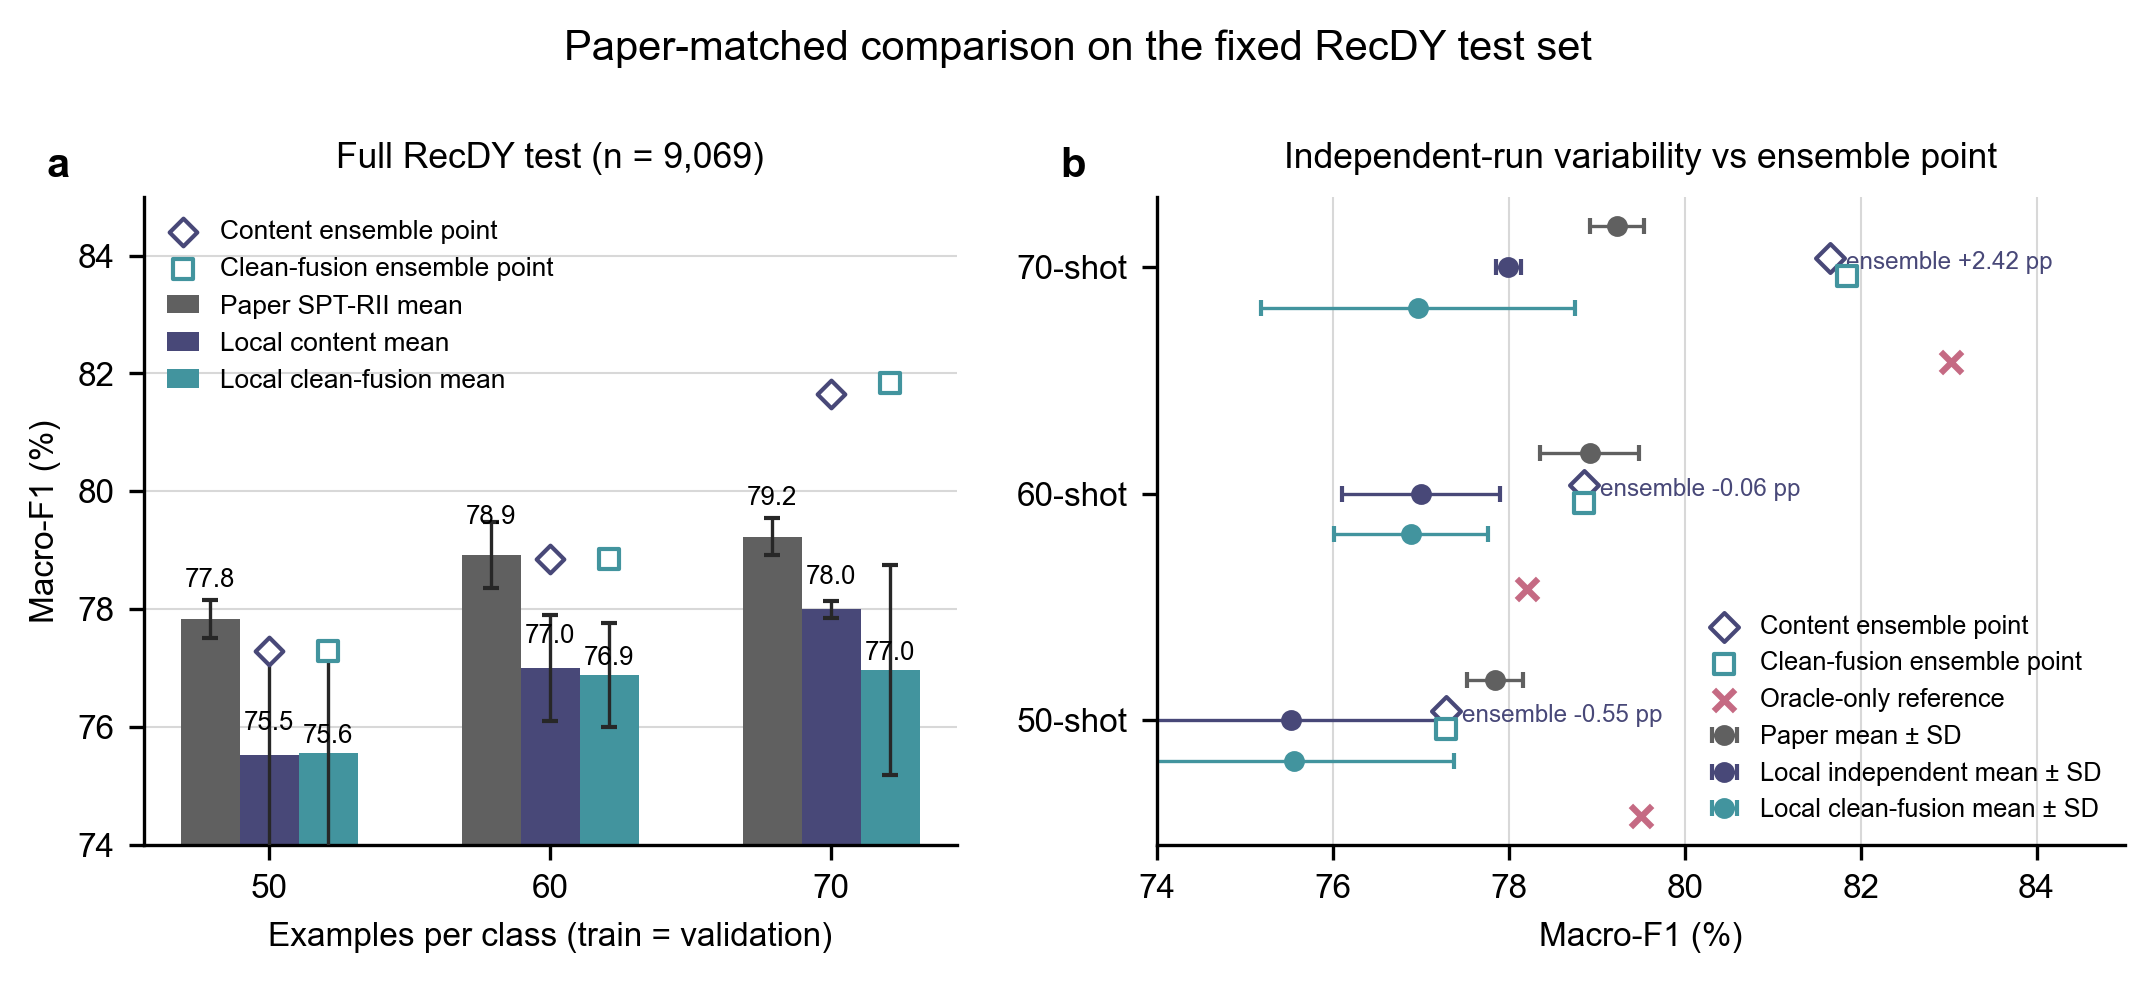
\includegraphics[width=\textwidth]{fig6_paper_comparison.png}
  \caption{固定 RecDY 测试集上的论文对齐比较。误差线为独立运行 SD；空心标记为单个集成点。}
  \label{fig:strict-comparison}
\end{figure}

\clearpage
\subsection{Table 5 四指标复核}

\begin{table}[H]
\centering
\small
\caption{原论文 Table~5 与本地结果的 Accuracy/Precision/Recall/F1 复核，单位为百分比。集成行是单点。}
\label{tab:four-metrics}
\begin{tabular}{clcccc}
\toprule
shot/类 & 方法 & Accuracy & Precision & Recall & F1 \\
\midrule
50 & 论文 SPT-RII & $78.41\pm0.39$ & $77.63\pm0.31$ & $78.96\pm0.20$ & $77.84\pm0.32$ \\
50 & 本地独立均值 & $76.59\pm2.37$ & $76.11\pm2.80$ & $75.74\pm1.03$ & $75.52\pm1.67$ \\
50 & 本地内容集成 & 78.21 & 77.17 & 77.44 & 77.29 \\
\addlinespace
60 & 论文 SPT-RII & $79.50\pm0.75$ & $78.65\pm0.49$ & $79.48\pm0.39$ & $78.92\pm0.56$ \\
60 & 本地独立均值 & $78.09\pm0.42$ & $77.21\pm0.31$ & $77.06\pm1.44$ & $77.00\pm0.89$ \\
60 & 本地内容集成 & 79.94 & 79.06 & 78.69 & 78.86 \\
\addlinespace
\rowcolor{LightBlue}70 & 论文 SPT-RII & $80.62\pm0.37$ & $79.96\pm0.32$ & $80.30\pm0.23$ & $79.23\pm0.31$ \\
70 & 本地独立均值 & $79.26\pm0.52$ & $78.63\pm0.92$ & $77.76\pm0.58$ & $78.00\pm0.14$ \\
\rowcolor{LightGold}70 & 本地内容集成 & 82.70 & 82.13 & 81.29 & 81.65 \\
70 & 严格固定 split 基线集成 & \StrictBaseAccuracy & \StrictBaseMacroPrecision & \StrictBaseMacroRecall & \StrictBaseEnsemble \\
70 & 严格 DAPT+R-Drop 同标签集成 & \StrictFullAccuracy & \StrictFullMacroPrecision & \StrictFullMacroRecall & \StrictFullEnsemble \\
\rowcolor{LightGreen}70 & 上述集成 + Qwen 选择性复核 & \QwenGateAccuracy & \QwenGatePrecision & \QwenGateRecall & \QwenGateFOne \\
\bottomrule
\end{tabular}
\end{table}

\begin{warningbox}[指标与论文内部不一致]
论文表头为 Prec./Rec./F1，但 \S6.4 未说明 averaging；本地三项采用宏平均。另有一处论文内部不一致：Table~5 的 RecDY 50-shot SPT-RII F1 为 $77.84\pm0.32\%$，Table~6 同一标签写 78.32\%。本文始终使用 Table~5 作为主参照。
\end{warningbox}

\clearpage
\section{严格同标注预算改进：DAPT + R-Drop}

\begin{infobox}[本轮新增协议]
从发布训练分区中用固定种子 20260718 抽取每类 70 条训练和每类 70 条验证；五个成员共享完全相同的 140 条训练行与 140 条验证行，只改变初始化和 Dropout。训练签名为
\texttt{f493253c...5ec7b}，验证签名为 \texttt{0725f080...8acd}；完整测试集仍为 9,069 条，阈值固定为 0.5，测试标签在所有 checkpoint 选择完成后才加载。
\end{infobox}

\subsection{改进方法与 4060 成本}

DAPT 阶段只读取训练分区的 \texttt{row\_id/content}，不读取人工标签、验证集或测试集。Chinese-RoBERTa 在
$\StrictDaptRows$ 条无标签弹幕上进行 1 epoch 掩码语言建模，mask 比例 0.15，最大长度 64，有效 batch 32；耗时
$\StrictDaptSeconds$ s，PyTorch 峰值显存 $\StrictDaptPeakGiB$ GiB。监督阶段最大 15 epoch、early stopping patience 4、学习率 $4\times10^{-5}$、最大长度 128；R-Drop 使用两次 dropout 前向、对称 KL 权重 0.5 和 0.05 label smoothing。DAPT 只覆盖 embeddings/encoder，原始 pooler 被明确保留，加载键审计为 197 个 encoder 键、0 个 unexpected key。

\begin{table}[H]
\centering
\small
\caption{固定同一标签集的 2$\times$2 消融。单成员 SD 仅表示固定 split 下的初始化/Dropout 波动；集成是单点。``对论文''与``对基线''均为百分点。}
\label{tab:same-budget-factorial}
\begin{tabular}{lccrrrr}
\toprule
方法 & DAPT & R-Drop & 单成员均值$\pm$SD & 同标签集成 & 对论文 & 对基线\\
\midrule
基础 RoBERTa + CE & 否 & 否 & 77.61$\pm$1.44 & 79.15 & -0.08 & +0.00\\
DAPT RoBERTa + CE & 是 & 否 & 79.23$\pm$1.07 & 80.45 & +1.22 & +1.30\\
基础 RoBERTa + R-Drop & 否 & 是 & 77.77$\pm$1.12 & 79.38 & +0.15 & +0.23\\
\rowcolor{LightGreen}DAPT RoBERTa + R-Drop & 是 & 是 & 80.01$\pm$0.62 & 80.60 & +1.37 & +1.45\\
\bottomrule
\end{tabular}

\end{table}

DAPT 是主要增益来源：仅 DAPT 已把同标签集成从 $\StrictBaseEnsemble\%$ 提高到 $80.45\%$；仅 R-Drop 为 $79.38\%$。二者结合后，五个单成员均值达到
$\StrictFullMemberMean\pm\StrictFullMemberSD\%$，相对固定 split 基线均值提高 $\StrictPairedMeanDelta$\pp；同标签五模型集成为 $\StrictFullEnsemble\%$，相对本地基线集成提高 $\StrictFullEnsembleBaseDelta$\pp，相对论文报告点高 $\StrictFullEnsemblePaperDelta$\pp。

\subsection{逐初始化配对与不确定性}

\begin{table}[H]
\centering
\small
\caption{同一标签集、同一初始化种子的逐成员配对结果。五个差值全部为正。}
\label{tab:same-budget-members}
\begin{tabular}{rrrr}
\toprule
初始化种子 & 基线 Macro-F1 & DAPT+R-Drop Macro-F1 & 配对差值（pp）\\
\midrule
100 & 78.76 & 80.09 & +1.33\\
101 & 75.47 & 80.37 & +4.90\\
102 & 76.77 & 78.92 & +2.15\\
103 & 78.43 & 80.30 & +1.87\\
104 & 78.61 & 80.38 & +1.77\\
\midrule
均值$\pm$SD & 77.61$\pm$1.44 & 80.01$\pm$0.62 & +2.40\\
\bottomrule
\end{tabular}

\end{table}

五个配对差值的均值为 $\StrictPairedMeanDelta$\pp，配对 $t$ 区间为
$[\StrictPairedCILow,\StrictPairedCIHigh]$\pp（$p=\StrictPairedTPValue$）。但 $n=5$ 很小，精确双侧符号检验为
$p=\StrictSignPValue$，因此不把单一参数检验写成最终显著性结论。对五成员集成做 5,000 次重采样时，结果如下。

\begin{table}[H]
\centering
\small
\caption{DAPT+R-Drop 同标签集成相对固定 split 基线集成的 paired bootstrap。}
\label{tab:same-budget-bootstrap}
\begin{tabular}{lrrr}
\toprule
重采样单位 & 集成差值（pp） & 95\% CI（pp） & $P(\Delta\leq0)$\\
\midrule
逐行 & +1.45 & [+0.85, +2.06] & 0.0000\\
按直播间聚类（12 组） & +1.45 & [+0.77, +2.45] & 0.0000\\
\bottomrule
\end{tabular}

\end{table}

逐行区间为 $[\StrictRowBootstrapLow,\StrictRowBootstrapHigh]$\pp，按 12 个直播间聚类后的区间为
$[\StrictClusterBootstrapLow,\StrictClusterBootstrapHigh]$\pp，均未跨 0。这支持“新方法相对本地同协议基线有增益”；相对论文的差值仍只能描述性解释，因为论文未公开逐样本预测且未说明 F1 averaging。

\begin{warningbox}[成立范围]
严格实验保持人工标签不变，但不是同计算/同数据预算：DAPT 额外读取 $\StrictDaptRows$ 条无标签训练文本，五模型集成约需单模型 5 倍计算。发布划分中还有 $\StrictTestExactOverlapRows$ 条测试弹幕与训练分区存在完全相同的表面文本（$\StrictTestExactOverlapPercent\%$）；DAPT 没有读取测试文件，但该重复限制了“全新文本泛化”的强主张。此外，本项目此前已观察过公开测试集，因此本轮属于锁定协议后的探索性验证，不是形式上的盲测。
\end{warningbox}

\clearpage
\section{必须使用大模型的完整改进：Qwen 选择性证据复核}

\begin{keybox}[本轮真正加入大模型后的主结果]
冻结的 \QwenGateModel 不做全量直接分类，也不把长解释强行拼入 RoBERTa。它只复核 DAPT+R-Drop 集成拿不准的样本，并且只有“多视角共识、置信度达标、证据可在当前弹幕逐字找到”同时成立时才允许改写预测。完整测试集 Macro-F1 从 $\QwenGateBaseFOne\%$ 提高到 $\QwenGateFOne\%$，大模型带来的本地增量为 $\QwenGateLocalDelta$\pp。
\end{keybox}

\subsection{相对原论文的方法改进}

原论文 \S5.2--5.3/Fig.~5 的做法是：对\emph{每条}弹幕读取前 20 条上下文，由 LLM 生成语义解释 $E_t$，再把原文与解释拼接后送入 soft prompt 模型。原论文 Table~6 的 Qwen3:8B 则使用 1,000 个样本做 PEFT，并作为独立分类器。本地实验把大模型改成第三种角色：\textbf{检索约束、可拒答的选择性复核器}。

\begin{table}[H]
\centering
\footnotesize
\caption{原论文大模型用法与本地完整方法的逐项对应。最后一行明确了本实验没有覆盖的论文组件。}
\label{tab:qwen-method-map}
\begin{tabularx}{\textwidth}{p{2.15cm}X X X}
\toprule
对照维度 & 原论文 \S5.2--5.3 / Fig.~5 & 本地选择性 Qwen & 改进及边界 \\
\midrule
大模型角色 & 为每条弹幕生成语义解释 & 只复核学生模型低置信样本 & 从全量特征生成改为选择性决策复核 \\
时序上下文 & 前 20 条弹幕用于解释生成 & 前 20 条只用于指代和语境消歧 & 最终证据仍必须来自当前弹幕 \\
领域锚点 & 解释文本与动态 verbalizer & 每类检索 \QwenGateRetrievalPerClass 条严格训练样本 & 不增加人工标签，但会重复使用已有标签 \\
输出约束 & 自由生成解释文本 & JSON 标签、置信度、原文证据、弃权标志 & 无合法证据即不能覆盖学生 \\
稳健性机制 & 解释生成一次后直接拼接 & 显式行为、潜在意图、负向过滤三视角投票 & 前两票高置信一致时早停，否则调用第三票 \\
融合方式 & 原文与解释拼接后送入 soft prompt & 仅在门控触发且至少两票一致时改写预测 & 无共识时自动保留学生答案 \\
大模型覆盖 & 原则上覆盖全部弹幕 & 只覆盖完整测试集的 $\QwenGateCandidatePercent\%$ & 节省调用，但不是无成本 \\
流式词表更新 & 动态 verbalizer 与半衰期更新 & 当前没有在线词表更新 & 不能宣称解决原论文的概念漂移问题 \\
\bottomrule
\end{tabularx}
\end{table}

设五模型平均的正类概率为 $\bar p_t$，验证集锁定的门控半宽为 $\delta=\QwenGateMargin$，则
\begin{equation}
G_t=\mathbb{I}\!\left(\left|\bar p_t-0.5\right|\leq\delta\right),\qquad
\hat y_t=
\begin{cases}
\hat y_t^{\mathrm{Qwen}}, & G_t=1\ \land\ A_t=1,\\
\mathbb{I}(\bar p_t\geq0.5), & \text{otherwise}.
\end{cases}
\label{eq:qwen-gate}
\end{equation}
其中 $A_t=1$ 要求至少两种视角给出同一标签、支持票平均置信度不低于 $\QwenGateMinConfidence$，且证据是当前弹幕的原文子串。每次调用提供前 $\QwenGateContextWindow$ 条无标签上下文和每类 \QwenGateRetrievalPerClass 条严格训练示例；生成配置固定为 temperature 0、\texttt{think=false}、\texttt{num\_predict=64}、\texttt{num\_ctx=2048}。

\subsection{验证集选门与测试标签隔离}

门控半宽只在锁定的 140 条验证集上选择。无门控时验证 Macro-F1 为 $\QwenGateValidationBase\%$，候选区间在相同验证集上扫描后选择 $\delta=\QwenGateMargin$，对应 $\QwenGateValidationFull\%$；这两个数只用于选规则，\textbf{不是最终性能结论}。选定后冻结提示词、模型 digest、解析器、检索数、三视角 reducer 和输入签名，再运行完整 9,069 条测试集；测试标签只在预测与选择文件落盘之后加载。协议哈希前缀为 \texttt{\QwenGateProtocolHashShort}，模型 digest 前缀为 \texttt{\QwenGateDigestShort}。

\begin{warningbox}[验证集也可能过拟合]
验证集只有 140 条，且 $\delta$ 来自多候选扫描，因此 $\QwenGateValidationFull\%$ 不能与论文或测试结果直接比较。本报告只把冻结后完整测试集的 $\QwenGateFOne\%$ 当作结果，并单独报告配对 bootstrap。
\end{warningbox}

\subsection{完整测试集结果与原论文对比}

\begin{table}[H]
\centering
\scriptsize
\caption{大模型相关主结果。论文两行取自原文 Table~5（p.14）和 Table~6（p.16）；本地两行使用同一固定人工标签集和同一测试集。本地 Prec./Rec./F1 为宏平均，论文 averaging 未说明。}
\label{tab:qwen-main-comparison}
% Local selective-Qwen delta: +0.34 pp; descriptive delta versus Paper Table 5: +1.71 pp.
\begin{tabularx}{\textwidth}{p{1.55cm}p{2.75cm}p{2.35cm}Xrrrr}
\toprule
来源 & 方法 & 人工监督 & 大模型角色 & Acc. & Prec. & Rec. & F1 \\
\midrule
论文 Table~5 & SPT-RII 70-shot & 70-shot；等大验证集 & 逐条生成解释并输入提示模型 & $80.62\pm0.37$ & $79.96\pm0.32$ & $80.30\pm0.23$ & $79.23\pm0.31$ \\
论文 Table~6 & Qwen3:8B PEFT & 1,000 样本 & 微调后的独立分类器 & 76.11 & 75.04 & 75.54 & 75.24 \\
本地严格实验 & DAPT+R-Drop 集成 & 70/类训练与验证 & 推理期不用大模型 & 81.55 & 80.73 & 80.48 & 80.60\\
\rowcolor{LightGreen}本地完整方法 & DAPT+R-Drop + 选择性 Qwen & 同一人工标签集 & 只复核低置信样本 & 82.10 & 81.61 & 80.49 & 80.94\\
\bottomrule
\end{tabularx}

\end{table}

选择性 Qwen 的 Accuracy、Macro-Precision、Macro-Recall 和 Macro-F1 分别为 $\QwenGateAccuracy\%$、$\QwenGatePrecision\%$、$\QwenGateRecall\%$ 和 $\QwenGateFOne\%$。与同一逐行预测上的无大模型学生相比，Macro-F1 提高 $\QwenGateLocalDelta$\pp；与论文 Table~5 的 SPT-RII 70-shot 报告点相比，描述性差值为 $\QwenGatePaperDelta$\pp。

相对论文 Table~6 的 Qwen3:8B PEFT 行，数值差为 $\QwenGatePaperQwenDelta$\pp，但这\textbf{不能解释为“本地 Qwen 本身高了 5.70 个百分点”}：Table~6 是 1,000 样本 PEFT 的独立分类器，而本地结果是 DAPT+R-Drop 学生与冻结 Qwen 复核器组成的系统，标签预算、模型角色和指标定义均不同。

\begin{figure}[H]
  \centering
  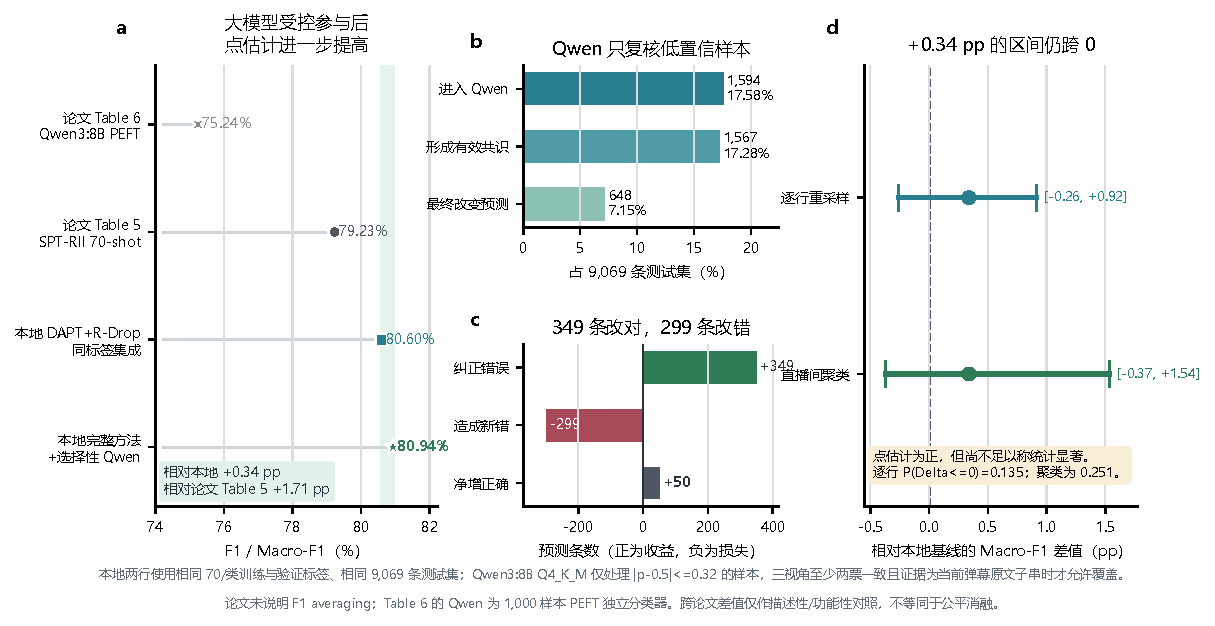
\includegraphics[width=\textwidth]{fig9_qwen_gate_comparison.pdf}
  \caption{选择性 Qwen 完整结果。a，论文 Table~5/Table~6 与本地学生/完整方法的性能点；b，只有低置信样本进入 Qwen；c，改对、改错和净增正确项；d，相对本地学生的逐行与直播间聚类 paired bootstrap 区间。两条区间均跨 0。}
  \label{fig:qwen-gate-comparison}
\end{figure}

\subsection{Qwen 到底改对了多少}

\begin{table}[H]
\centering
\small
\caption{选择性复核的路由与错误账本。百分比均以完整 9,069 条测试集为分母，除最后一列外。}
\label{tab:qwen-routing}
\begin{tabular}{lrrr}
\toprule
路由阶段或结果 & 条数 & 占测试集 & 占改写预测 \\
\midrule
完整测试集 & 9,069 & 100.00\% & --\\
进入 Qwen 的低置信样本 & 1,594 & 17.58\% & --\\
Qwen 形成有效共识 & 1,567 & 17.28\% & --\\
最终改变小模型预测 & 648 & 7.15\% & 100.00\%\\
其中：纠正原错误 & 349 & 3.85\% & 53.86\%\\
其中：破坏原正确项 & 299 & 3.30\% & 46.14\%\\
\rowcolor{LightGreen}净增加正确预测 & +50 & +0.55\% & --\\
\bottomrule
\end{tabular}

\end{table}

完整测试集中有 $\QwenGateCandidateRows$ 条进入 Qwen，$\QwenGateConsensusRows$ 条形成有效共识，最终有 $\QwenGateChangedRows$ 条改变学生预测。Qwen 纠正 $\QwenGateCorrectedRows$ 个基线错误，同时破坏 $\QwenGateHarmedRows$ 个原本正确的样本，净增加 $\QwenGateNetRows$ 个正确预测。这个账本说明大模型确实提供了互补判断，但其意见并非天然可靠；证据校验、共识与保留学生答案都是必要的保险。

\subsection{统计边界：有正向点估计，尚无稳健显著性}

\begin{table}[H]
\centering
\small
\caption{选择性 Qwen 相对本地 DAPT+R-Drop 集成的 5,000 次 paired bootstrap。}
\label{tab:qwen-bootstrap}
\begin{tabular}{lrrr}
\toprule
重采样单位 & 点差（pp） & 95\% CI（pp） & $P(\Delta\leq0)$ \\
\midrule
逐行 & $\QwenGateLocalDelta$ & $[\QwenGateRowCILow,\QwenGateRowCIHigh]$ & \QwenGateRowPNonPositive \\
按 \texttt{live\_id} 聚类（12 组） & $\QwenGateLocalDelta$ & $[\QwenGateClusterCILow,\QwenGateClusterCIHigh]$ & \QwenGateClusterPNonPositive \\
\bottomrule
\end{tabular}
\end{table}

两条 95\% 区间都跨 0，所以本轮可以说“Qwen 将点估计从 $\QwenGateBaseFOne\%$ 进一步推到 $\QwenGateFOne\%$”，但不能说“Qwen 已显著提高性能”。跨论文的 $\QwenGatePaperDelta$\pp 更不能做显著性检验，因为原论文没有公开逐行预测，且 F1 averaging 未说明。

\subsection{RTX 4060 可运行性与额外成本}

Qwen 只覆盖 $\QwenGateCandidatePercent\%$ 的测试样本，但每个候选需要 2--3 个视角。缓存中成功记录的推理时间累计约 $\QwenGateRecordedMinutes$ min；正式重建阶段利用缓存，只重试 \QwenGateNewRetryRecords 条无效记录，用时 $\QwenGateFormalRetrySeconds$ s。该计时不等同于论文 Table~9 的“单条解释生成时间”，也不包含学生模型训练。正式重建的显存监控没有捕获有效峰值；同一量化模型在此前直接调用中测得约 6.40 GiB，说明 8 GB RTX 4060 可以运行，但全量实验仍需约 1.5--2 h 的大模型推理时间。

\begin{riskbox}[当前结论的准确写法]
“在固定同一份 70-shot/类人工标签和完整 RecDY 测试集上，DAPT+R-Drop 同标签集成为 $\QwenGateBaseFOne\%$ Macro-F1；加入证据约束的 Qwen3:8B 选择性复核后，点估计提高到 $\QwenGateFOne\%$。该完整系统描述性高于论文 Table~5 的 $\StrictPaperFOne\%$，但 Qwen 的额外 $\QwenGateLocalDelta$\pp 增量区间跨 0，仍需未触碰测试集确认。”
\end{riskbox}

\clearpage
\section{内部提升：对应 \S5.3、\S6.6 Fig.6，但协议不同}

\begin{infobox}[可比性等级：C]
以下实验使用 400 条固定本地测试子集，训练规模为 400 或 1,000。它们用于判断本地改进是否有效，不能把绝对 F1 直接减去论文 Table~5。
\end{infobox}

\subsection{字符 TF--IDF：解释分通道与 OOF 晚期融合}

\begin{table}[H]
\centering
\small
\caption{TF--IDF 改进实验。置信区间为测试样本配对 bootstrap；跨 0 表示证据尚不足。}
\label{tab:tfidf-improvement}
\begin{tabularx}{\textwidth}{c X c c X}
\toprule
训练量 & 方法 & Macro-F1 & 相对基线 & 不确定性/备注 \\
\midrule
400 & 内容基线 & 78.88\% & 基准 & -- \\
400 & 旧 Qwen 解释直接拼接 & 80.75\% & $+1.87$\pp & 95\% CI $[-2.80,+6.69]$ \\
400 & 结构化解释直接拼接 & 80.84\% & $+1.96$\pp & 相对旧提示仅 $+0.09$\pp \\
\rowcolor{LightGreen}400 & 旧解释 + OOF 晚期融合 & 82.39\% & $+3.51$\pp & 95\% CI $[-0.32,+7.35]$ \\
400 & 结构化解释 + OOF 晚期融合 & 80.03\% & $+1.14$\pp & 95\% CI $[-1.00,+3.41]$ \\
\addlinespace
1000 & 内容基线 & 82.29\% & 基准 & -- \\
1000 & 结构化解释直接拼接 & 82.94\% & $+0.65$\pp & -- \\
\rowcolor{LightGreen}1000 & 结构化解释 + OOF 晚期融合 & 83.82\% & $+1.53$\pp & 95\% CI $[-1.28,+4.34]$ \\
\bottomrule
\end{tabularx}
\end{table}

数据量和融合策略有价值，但“改成结构化提示”本身没有稳定胜过旧提示。400 条时旧解释 late fusion 最强；1,000 条时结构化 late fusion 相对内容基线提高 1.53\pp。

\subsection{RoBERTa：compact explanation 与验证集融合}

\begin{table}[H]
\centering
\small
\caption{RoBERTa 三种子结果。1000 条 compact late fusion 的逐种子提升为 $+0.154/+0.746/+0.401$\pp。}
\label{tab:roberta-improvement}
\begin{tabularx}{\textwidth}{c X c c X}
\toprule
训练量 & 输入/融合 & Macro-F1 均值$\pm$SD & 相对内容基线 & 判断 \\
\midrule
400 & 内容基线 & $84.90\pm1.52\%$ & 基准 & -- \\
400 & 旧 Qwen 直接拼接 & $82.57\pm0.67\%$ & $-2.34$\pp & 退化 \\
400 & 结构化解释直接拼接 & $82.44\pm1.66\%$ & $-2.46$\pp & 退化 \\
400 & compact 直接拼接 & $84.30\pm1.75\%$ & $-0.60$\pp & 基本追回 \\
400 & compact late fusion & $84.88\pm0.61\%$ & $-0.03$\pp & 种子方向不一致 \\
\addlinespace
1000 & 内容基线 & $87.19\pm0.53\%$ & 基准 & -- \\
1000 & 结构化解释直接拼接 & $86.73\pm1.12\%$ & $-0.46$\pp & 仍退化 \\
1000 & compact 直接拼接 & $87.21\pm0.51\%$ & $+0.02$\pp & 接近持平 \\
\rowcolor{LightGreen}1000 & compact late fusion & $87.63\pm0.29\%$ & $+0.43$\pp & 三个种子均为正 \\
\bottomrule
\end{tabularx}
\end{table}

RoBERTa 对噪声解释敏感。长解释直接拼接会破坏内容信号；缩短解释并改为 late fusion 后，1,000 条训练下得到小幅且三个种子同方向的提升，但 $n=3$ 仍不足以声称统计显著。

\begin{figure}[H]
  \centering
  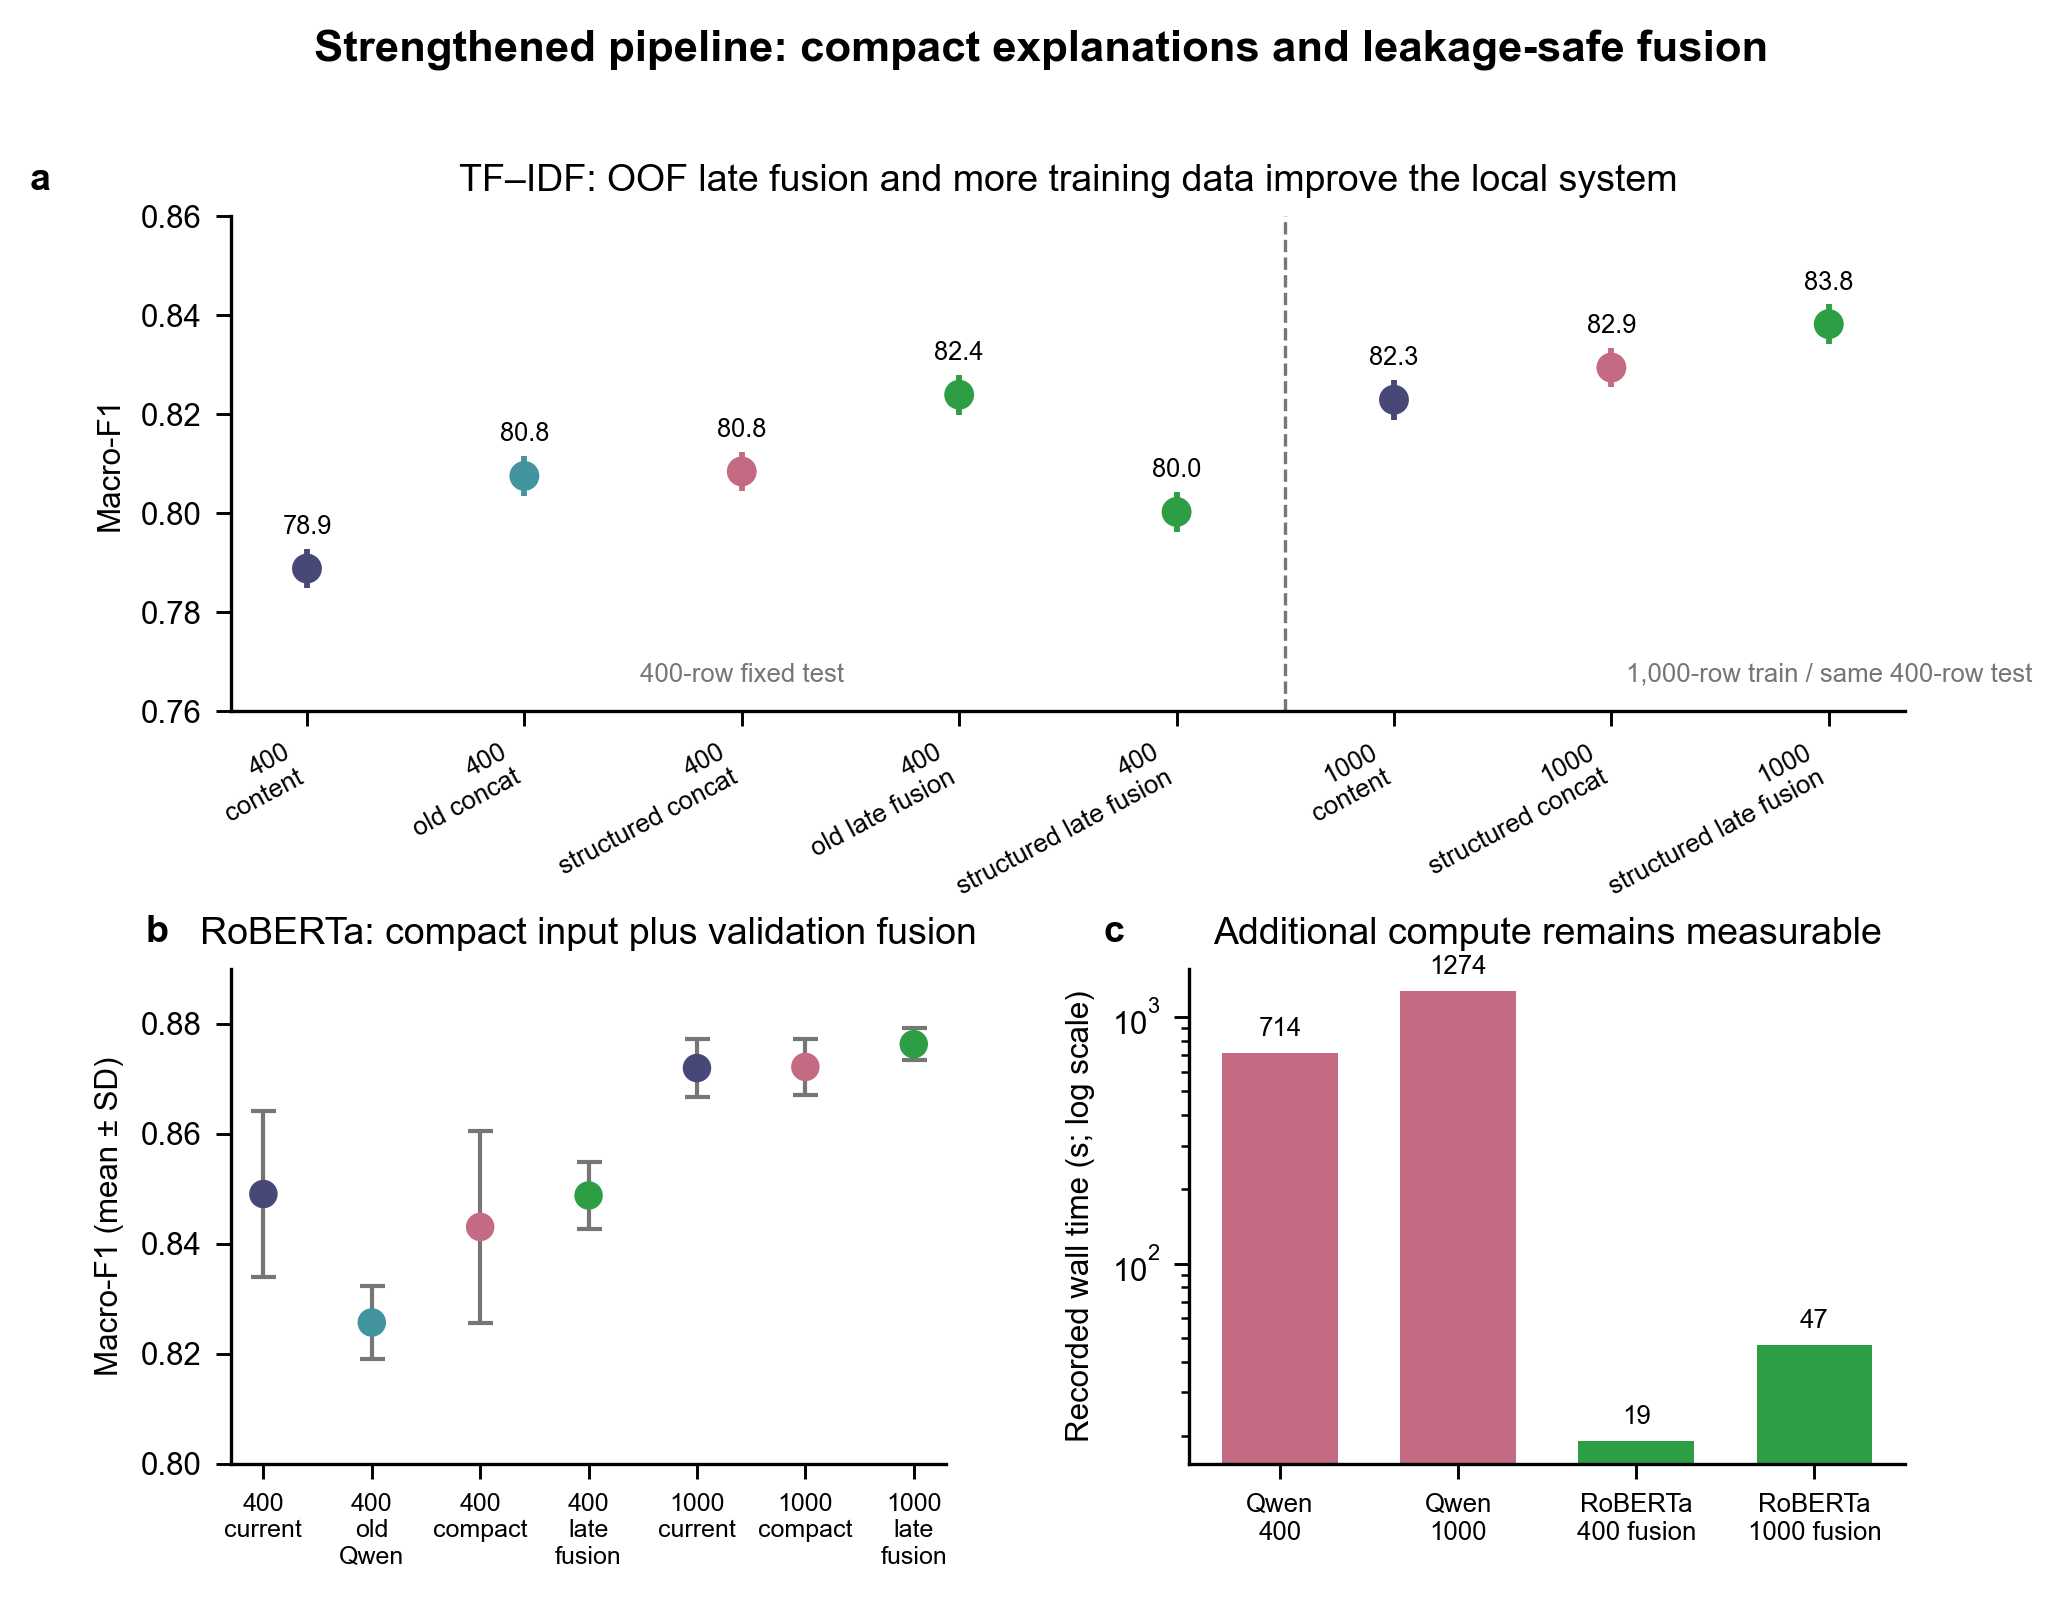
\includegraphics[width=0.98\textwidth]{fig5_improvement_results.png}
  \caption{内部改进总览：TF--IDF、RoBERTa 与额外计算开销。误差线定义见原实验记录。}
  \label{fig:internal-improvement}
\end{figure}

\subsection{与原论文 Fig.6 的对应方式}

\begin{table}[H]
\centering
\small
\caption{原论文 Fig.6 与本地内部消融的概念映射。绝对值不作横向胜负比较。}
\label{tab:fig6-map}
\begin{tabularx}{\textwidth}{X c c X}
\toprule
实验 & F1/Macro-F1 & 组件变化 & 比较边界 \\
\midrule
原论文完整 SPT-RII & 78.3\% & -- & 同一 SPT-RII 框架 \\
原论文 $-$explanations & 74.0\% & $-4.3$\pp & 证明解释模块重要 \\
原论文 $-$update & 75.5\% & $-2.8$\pp & 证明动态更新重要 \\
本地 TF--IDF 1000 late fusion & 83.82\% & $+1.53$\pp vs 本地内容 & 不同模型/测试子集 \\
本地 RoBERTa 1000 compact late fusion & $87.63\pm0.29\%$ & $+0.43$\pp vs 本地内容 & 不同模型/测试子集 \\
\bottomrule
\end{tabularx}
\end{table}

\clearpage
\section{前期小样本门控探索：对应 \S6.7 / Table 6}

本节保留在正式严格实验之前完成的 400 条子集探索，用于说明方案是如何形成的；它\textbf{不是当前主结果}。原论文 Table~6 比较了 10-shot LLM、1,000 样本 PEFT 与 SPT-RII。该前期实验没有让 Qwen 全量替代分类器，而只处理 TF--IDF 置信度落在 $[0.28,0.72]$ 的样本；阈值在 200 条验证集上选择，测试子集评估一次。正式 9,069 条测试结果见图~\ref{fig:qwen-gate-comparison} 与表~\ref{tab:qwen-main-comparison}。

\begin{table}[H]
\centering
\small
\caption{不确定性门控结果。提升区间跨 0，因此属于探索性证据。}
\label{tab:gate-comparison}
\begin{tabular}{lcccc}
\toprule
方法 & Macro-F1 & 测试数 & Qwen 覆盖 & 相对基线 \\
\midrule
TF--IDF 基线 & 82.29\% & 400 & 0\% & 基准 \\
Qwen 直接分类 & 74.70\% & 400 & 100\% & 单独使用更差 \\
\rowcolor{LightGreen}不确定性门控 & 83.71\% & 400 & 38.5\% & $+1.42$\pp；95\% CI $[-2.61,+5.37]$ \\
\bottomrule
\end{tabular}
\end{table}

154 条被路由样本上，Qwen 纠正 33 个基线错误，同时破坏 28 个原本正确样本，净增 5 条正确预测。混淆矩阵从 $[[120,37],[30,213]]$ 变为 $[[125,32],[30,213]]$，主要减少 5 个负类被误报为正类的错误。

\begin{figure}[H]
  \centering
  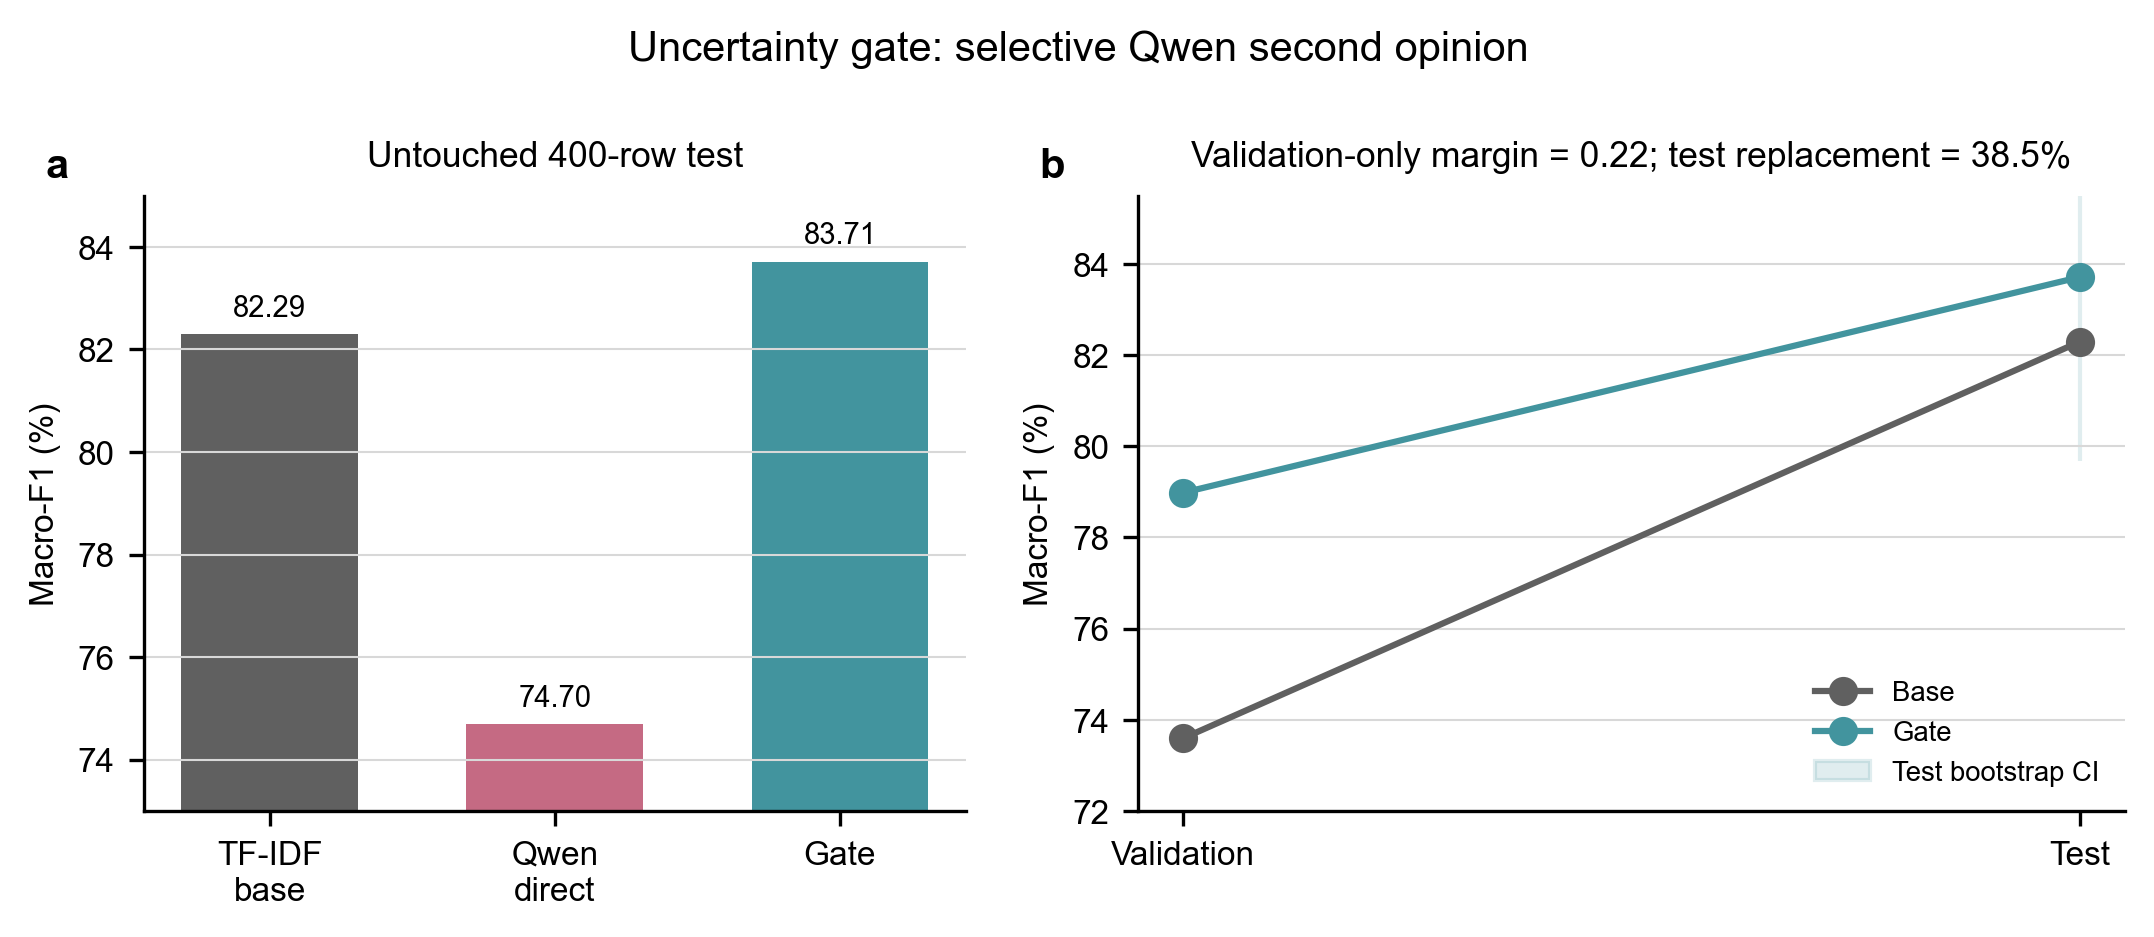
\includegraphics[width=\textwidth]{fig7_uncertainty_gate.png}
  \caption{不确定性门控：验证集选阈值，固定测试集一次评估。}
  \label{fig:gate}
\end{figure}

\begin{riskbox}[为什么不能与 Table 6 直接相减]
论文 Table~6 的大模型行是另一套 few-shot/PEFT 条件；本节门控只在 400 条子集上评估，还把 TF--IDF 与 Qwen 组合。83.71\% 不能写成“比论文 SPT-RII 78.32\% 高 5.39\pp”，也不能替代当前严格同标签预算的 $\QwenGateFOne\%$ 主结果。
\end{riskbox}

\section{效率：对应 \S6.10 / Table 9 / p.17}

\begin{table}[H]
\centering
\small
\caption{原论文 Table~9 与本地生成开销。硬件、量化、计时范围和任务均不同。}
\label{tab:efficiency}
\begin{tabularx}{\textwidth}{c l c c c X}
\toprule
来源 & 模型 & 报告 F1 & 时间 & 硬件 & 任务含义 \\
\midrule
论文 & Llama3.1-8B & 75.79\% & 257 ms/条 & RTX 4090 & 作为 SPT-RII 解释器 \\
论文 & Qwen2.5-7B & 76.74\% & 283 ms/条 & RTX 4090 & 作为 SPT-RII 解释器 \\
论文 & Deepseek-V3 & 78.32\% & 985 ms/条 & 未单列 & 远程/大模型设置 \\
论文 & ChatGPT-3.5 & 79.09\% & 1072 ms/条 & 服务端 & 远程 API \\
论文 & ChatGPT-4o & 78.60\% & 1062 ms/条 & 服务端 & 远程 API \\
\rowcolor{LightGold}本地 & Qwen3-8B Q4 & 非同一 F1 & 562 ms/条 & RTX 4060 8 GB & 800 条墙钟 450.2 s；峰值 6.40 GiB \\
\rowcolor{LightGreen}本地严格 & \QwenGateModel & \QwenGateFOne\% & 累计约 \QwenGateRecordedMinutes\ min & RTX 4060 8 GB & 路由 \QwenGateCandidateRows 条；每条 2--3 视角 \\
\bottomrule
\end{tabularx}
\end{table}

原论文 Table~9 测的是“更换 SPT-RII 解释生成模型后的整体 F1 和单条时间”；本地 0.562 s/条只统计早期 Qwen3-8B Q4 的解释生成，严格选择性复核的 \QwenGateRecordedMinutes\ min 是缓存中成功调用的累计推理时间。任务、提示长度、调用次数、量化和硬件都不同，因此这里只能证明 RTX 4060 可以跑通并量化本地成本，不能得出速度优越性结论。

\clearpage
\section{如何通俗解释这次提升}

\begin{keybox}[30 秒讲法]
可以把系统理解为“学生先答，老师只检查难题”。RoBERTa 先阅读训练分区无标签弹幕，熟悉直播语言，再用 R-Drop 稳住少样本学习；五模型学生集成为 $\QwenGateBaseFOne\%$。只有学生拿不准的 $\QwenGateCandidatePercent\%$ 样本才交给 Qwen，而且 Qwen 必须引用弹幕原话、至少两种视角一致，才有资格改答案。最终 Macro-F1 为 $\QwenGateFOne\%$，比学生高 $\QwenGateLocalDelta$\pp，比论文 Table~5 的 $\StrictPaperFOne\%$ 描述性高 $\QwenGatePaperDelta$\pp；但大模型这一小段增量的区间跨 0，所以应说“点估计更高”，不能说“已经显著提升”。
\end{keybox}

\begin{figure}[H]
  \centering
  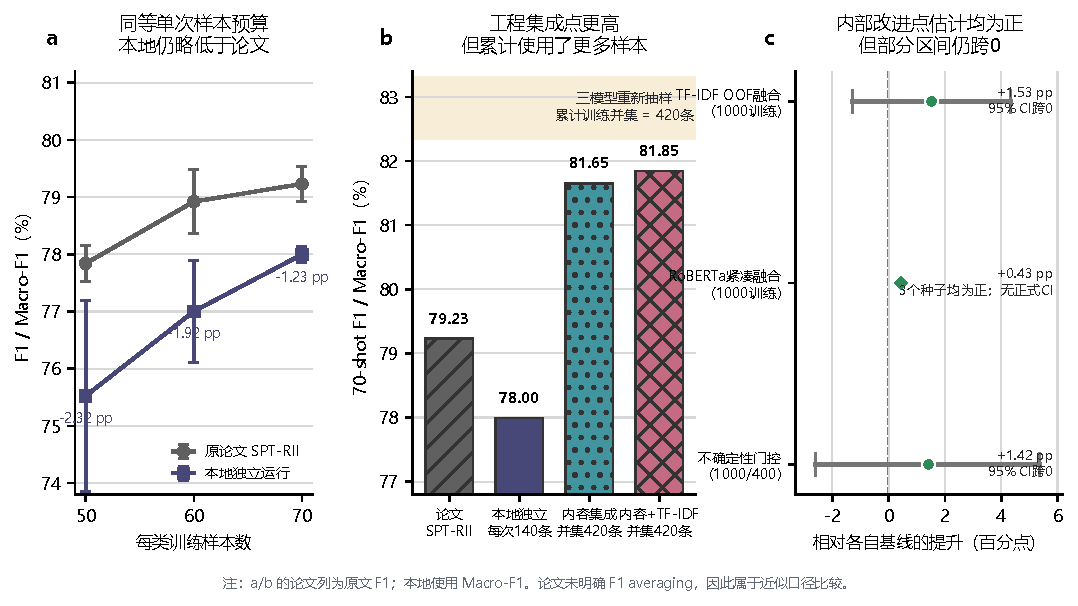
\includegraphics[width=\textwidth]{fig8_plain_comparison.pdf}
  \caption{面向汇报的严格同预算对照图。a，论文报告点、本地固定 split 初始化均值和同标签集成点；b，DAPT/R-Drop 的 2$\times$2 消融，主要增益来自 DAPT；c，五个同种子配对差值全部为正，并给出逐行与直播间聚类 bootstrap 区间。}
  \label{fig:plain-comparison}
\end{figure}

\clearpage
\subsection{按两张图讲四句话}

\begin{enumerate}[leftmargin=2.2em,itemsep=0.45em]
  \item \textbf{先讲标签预算。} 看图~\ref{fig:plain-comparison}a：五个成员使用相同的 140 条训练标签和 140 条验证标签；DAPT+R-Drop 单成员均值与同标签集成均越过论文 $\StrictPaperFOne\%$ 报告点。
  \item \textbf{再讲学生为什么变强。} 看图~\ref{fig:plain-comparison}b：只加 R-Drop 的集成提高 $0.23$\pp，只做 DAPT 已提高 $1.30$\pp，两者结合提高 $\StrictFullEnsembleBaseDelta$\pp。核心是先用无标签数据熟悉直播语言，再用一致性训练降低波动。
  \item \textbf{然后讲大模型怎么用。} 看图~\ref{fig:qwen-gate-comparison}b--c：Qwen 不做所有题，只复核 $\QwenGateCandidateRows$ 条低置信样本；它改对 $\QwenGateCorrectedRows$ 条、改错 $\QwenGateHarmedRows$ 条，净增加 $\QwenGateNetRows$ 条正确预测，最终把 $\QwenGateBaseFOne\%$ 推到 $\QwenGateFOne\%$。
  \item \textbf{最后讲证据边界。} 图~\ref{fig:plain-comparison}c 表明 DAPT+R-Drop 相对基础学生的区间未跨 0；但图~\ref{fig:qwen-gate-comparison}d 中 Qwen 额外增量的逐行区间 $[\QwenGateRowCILow,\QwenGateRowCIHigh]$\pp、聚类区间 $[\QwenGateClusterCILow,\QwenGateClusterCIHigh]$\pp 都跨 0。前者证据较稳，后者目前只是正向点估计。
\end{enumerate}

\begin{warningbox}[最容易讲错的地方]
\textbf{不建议说：}“我们完全复现并在所有条件下显著超过了 SPT-RII。”

\textbf{建议说：}“在固定同一份 70-shot/类人工标签后，DAPT+R-Drop 同标签集成为 $\QwenGateBaseFOne\%$；再让 Qwen 只复核低置信样本，完整方法达到 $\QwenGateFOne\%$。这比论文 Table~5 的 $\StrictPaperFOne\%$ 描述性高 $\QwenGatePaperDelta$ 个百分点。大模型确实让点估计再提高 $\QwenGateLocalDelta$ 个百分点，但其置信区间跨 0，因此还不能说额外提升已经显著。”
\end{warningbox}

\subsection{老师追问时的简短回答}

\begin{description}[leftmargin=1.0cm,itemsep=0.55em]
  \item[问：]为什么不能直接拿 83.82\% 或 87.63\% 与论文的 79.23\% 比？
  \item[答：]因为它们来自 1,000 条训练、400 条测试的内部实验，测试样本和训练预算都不同。只有完整 9,069 条测试集上的 50/60/70-shot 实验最接近论文 Table~5。
  \item[问：]现在能不能说对论文有进步？
  \item[答：]可以说“在同人工标签预算、完整 RecDY 测试集上，包含 Qwen 的完整系统达到 $\QwenGateFOne\%$，描述性超过论文报告点 $\StrictPaperFOne\%$”。不能说完整复现 SPT-RII，也不能说同计算/同总数据预算。
  \item[问：]大模型是不是被放弃了？
  \item[答：]没有。Qwen 从“每条都写解释”改成了“只审难题的复核器”。它实际处理 $\QwenGateCandidateRows$ 条样本，必须给出原文证据并形成多视角共识，最终净增加 $\QwenGateNetRows$ 条正确预测。
  \item[问：]这些提升算不算已经证明有效？
  \item[答：]要分两层。DAPT+R-Drop 相对本地基础学生的逐行和直播间聚类区间都未跨 0；Qwen 在其上额外增加的 $\QwenGateLocalDelta$\pp 区间跨 0，因此只能称正向点估计。公开测试集此前还被观察过，仍需未触碰数据确认。
  \item[问：]到底是 DAPT 还是 R-Drop 起作用？
  \item[答：]主要是 DAPT。集成层面只加 R-Drop 为 $+0.23$\pp，只加 DAPT 为 $+1.30$\pp，二者结合为 $\StrictFullEnsembleBaseDelta$\pp；R-Drop 更明显的作用是把单成员 SD 从 $1.44$ 降到 $0.62$ 个百分点。
  \item[问：]4060 能承担吗？
  \item[答：]可以。DAPT 用时 $\StrictDaptSeconds$ s、峰值 $\StrictDaptPeakGiB$ GiB；监督 R-Drop 单成员峰值约 2.16 GiB。Qwen 成功调用的累计推理时间约 $\QwenGateRecordedMinutes$ min，同量化模型此前直接调用峰值约 6.40 GiB。可以单卡顺序完成，但不是实时零成本方案。
\end{description}

\FloatBarrier
\section{可信度、限制与下一步}

\subsection{目前可以成立的结论}
\begin{itemize}[leftmargin=2em,itemsep=0.3em]
  \item 严格 70-shot 实验已固定同一组训练/验证行、五个初始化、阈值 0.5 和完整 9,069 条测试集；四个预注册消融条件均已报告，没有只挑最高条件。
  \item DAPT+R-Drop 单成员均值为 $\StrictFullMemberMean\pm\StrictFullMemberSD\%$，同标签集成为 $\StrictFullEnsemble\%$，相对本地固定 split 基线的配对 bootstrap 区间未跨 0。
  \item 冻结 Qwen3:8B 以检索增强、证据约束的选择性复核器参与完整测试；系统达到 $\QwenGateFOne\%$ Macro-F1，相对论文 Table~5 描述性高 $\QwenGatePaperDelta$\pp。
  \item 大模型相对本地学生的额外点差为 $\QwenGateLocalDelta$\pp；逐行和直播间聚类区间都跨 0，因此只称“进一步提高点估计”，不称统计显著。
  \item 2$\times$2 消融确认主要增益来自 DAPT；R-Drop 单独收益小，但与 DAPT 结合后进一步提高单成员均值并降低固定 split 下的初始化波动。
  \item 1,000 条训练时，TF--IDF late fusion 提高 1.53\pp；RoBERTa compact late fusion 提高 0.43\pp，三个种子方向一致。
  \item 路由账本显示 Qwen 改对 $\QwenGateCorrectedRows$ 条、改错 $\QwenGateHarmedRows$ 条、净增 $\QwenGateNetRows$ 条；选择性使用比前期全量直接分类更合理，但仍有明确副作用。
\end{itemize}

\subsection{不能忽略的限制}
\begin{table}[H]
\centering
\small
\caption{结果解释所需的边界条件。}
\label{tab:limitations}
\begin{tabularx}{\textwidth}{p{2.5cm}X X}
\toprule
风险 & 事实 & 文档处理 \\
\midrule
指标定义 & 论文未明确 F1 averaging；本地用 Macro-F1 & 所有跨论文差值标为近似口径 \\
方法完整性 & 未实现 soft prompt、BiLSTM、动态 verbalizer & 称为低成本替代，不称完整复现 \\
无标签数据预算 & DAPT 读取训练分区 $\StrictDaptRows$ 条无标签弹幕 & 称“同人工标签预算”，不称同总数据预算 \\
集成计算预算 & 五个成员共享标签，但约需单模型 5 倍微调/推理 & 同时报告单成员均值与集成单点 \\
大模型额外计算 & $\QwenGateCandidateRows$ 条候选各需 2--3 个视角；累计记录约 $\QwenGateRecordedMinutes$ min & 报告覆盖率、调用成本与缓存修复，不称免费提升 \\
门控选择 & 140 条验证集扫描不确定性区间，可能选择性过拟合 & 测试只在锁定后评估；仍需新验证集复核 \\
Qwen 增量功效 & $\QwenGateLocalDelta$\pp；逐行 CI $[\QwenGateRowCILow,\QwenGateRowCIHigh]$，聚类 CI $[\QwenGateClusterCILow,\QwenGateClusterCIHigh]$ & 只称正向点估计，不称显著提升 \\
测试历史 & 公开 RecDY 测试集此前已被本项目观察 & 定位为锁定协议后的探索性验证，不称正式盲测 \\
重复表面文本 & $\StrictTestExactOverlapRows$ 条测试弹幕与训练分区文本完全相同 & 限制“全新文本泛化”主张 \\
同直播间相关性 & 12 个 \texttt{live\_id} 同时出现在训练/测试 & 补充直播间聚类 bootstrap；仍需跨直播间留出 \\
统计功效 & 固定 split 只有 5 个初始化；符号检验 $p=\StrictSignPValue$ & 不把跨论文差值写成正式显著性结论 \\
\bottomrule
\end{tabularx}
\end{table}

\subsection{下一轮优先实验}
\begin{enumerate}[leftmargin=2.2em,itemsep=0.35em]
  \item 将已锁定的 DAPT+R-Drop + Qwen 完整规则原样运行在未触碰的平台或按 \texttt{live\_id} 完整留出的测试集，确认 $\QwenGateLocalDelta$\pp 是否可重复。
  \item 对 Qwen 组件做预注册消融：去检索示例、去原文证据检查、固定两票、固定三票、禁止上下文；验证收益究竟来自哪一项约束。
  \item 把严格协议扩展到 50/60-shot，验证相对论文 Table~5 的增益是否贯穿不同标注规模，而不是只出现在 70-shot。
  \item 比较单模型 checkpoint averaging、五模型集成与 Qwen 路由，绘制 Macro-F1--耗时曲线，争取把约 5 倍学生计算和 1.5--2 h 大模型推理压缩到可部署水平。
\end{enumerate}

\begin{keybox}[最终判断]
本轮已经形成一个\textbf{实际使用大模型}的完整系统：在固定同一份 70-shot/类人工标签后，DAPT+R-Drop 同标签集成为 $\QwenGateBaseFOne\%$，证据约束的 Qwen 选择性复核把点估计进一步提高到 $\QwenGateFOne\%$。该结果相对论文 Table~5 的 $\StrictPaperFOne\%$ 为描述性 $\QwenGatePaperDelta$\pp，但 Qwen 自身的 $\QwenGateLocalDelta$\pp 增量区间跨 0。最稳妥的表述是“在 RTX 4060 上，同人工标签预算的本地完整方法获得了高于论文报告点的受控结果，大模型带来额外正向点估计”；不能写成完整复现、同计算预算或显著击败 SPT-RII。
\end{keybox}

\section{证据文件索引}

以下路径对应本文全部数字和原文位置。\texttt{source\_map.json} 提供 S/T 锚点，CSV/JSON 文件提供本地逐种子、融合和门控证据。

\footnotesize
\begin{description}[leftmargin=3.0cm,labelwidth=2.6cm,style=nextline,itemsep=0.16em,topsep=0.20em]
  \item[原论文 PDF] \path{E:\zotero\storage\7DATFQRR\Zhu }等\path{ - 2026 - Analyzing bullet chats for recommendation intent identification Dataset and method.pdf}
  \item[原文位置映射] \path{E:\Lab\experiment\paper_reader\source_map.json}
  \item[Table 5 原图] \path{E:\Lab\experiment\paper_reader\assets\table5_recdy.png}
  \item[Table 5 对比目录] \path{E:\Lab\experiment\results\paper_comparison}
  \item[历史内部实验目录] \path{E:\Lab\experiment\results\improvement}
  \item[严格协议清单] \path{E:\Lab\experiment\config\same_budget_protocol_v1.json}
  \item[DAPT 无标签适配] \path{E:\Lab\experiment\results\same_budget\dapt_result.json}
  \item[严格四条件汇总] \path{E:\Lab\experiment\results\same_budget\strict70_analysis.json}
  \item[严格逐成员指标] \path{E:\Lab\experiment\results\same_budget\strict70_member_metrics.csv}
  \item[严格 bootstrap] \path{E:\Lab\experiment\results\same_budget\strict70_bootstrap.csv}
  \item[严格对照图源数据] \path{E:\Lab\experiment\figures\source_data_fig8.csv}
  \item[Qwen 验证锁定] \path{E:\Lab\experiment\results\same_budget\strict70_qwen_gate_selection.json}
  \item[Qwen 正式结果] \path{E:\Lab\experiment\results\same_budget\strict70_qwen_gate_result.json}
  \item[Qwen 统计分析] \path{E:\Lab\experiment\results\same_budget\strict70_qwen_gate_analysis.json}
  \item[Qwen 逐行预测] \path{E:\Lab\experiment\results\same_budget\strict70_qwen_gate_predictions.csv}
  \item[Qwen 改写样本] \path{E:\Lab\experiment\results\same_budget\strict70_qwen_gate_changed_cases.csv}
  \item[Qwen 对照图源数据] \path{E:\Lab\experiment\figures\source_data_fig9.csv}
\end{description}
\normalsize

\vfill
\begin{center}
\small\color{Muted}文档版本：2026-07-19。主源文件：\texttt{improvement\_comparison.tex}。
\end{center}

\end{document}
